%# -*- coding: utf-8-unix -*-
%%==================================================
%% thesis.tex
%%==================================================

% 双面打印
\documentclass[master, fontset=adobe, openright, twoside]{sjtuthesis}
% \documentclass[bachelor, fontset=adobe, openany, oneside, submit]{sjtuthesis} 
% \documentclass[master, adobefonts, review]{sjtuthesis} 
% \documentclass[%
%   bachelor|master|doctor,	% 必选项
%   fontset=adobe|windows,  	% 只测试了adobe
%   oneside|twoside,		% 单面打印,双面打印(奇偶页交换页边距,默认)
%   openany|openright, 		% 可以在奇数或者偶数页开新章|只在奇数页开新章(默认)
%   zihao=-4|5,, 		% 正文字号:小四、五号(默认)
%   review,	 		% 盲审论文,隐去作者姓名、学号、导师姓名、致谢、发表论文和参与的项目
%   submit			% 定稿提交的论文,插入签名扫描版的原创性声明、授权声明 
% ]

% 逐个导入参考文献数据库
\addbibresource{bib/thesis.bib}
% \addbibresource{bib/chap2.bib}

\begin{document}

%\bibliographystyle{plain}
%% 无编号内容:中英文论文封面、授权页
%# -*- coding: utf-8-unix -*-
\title{上海交通大学学位论文 \LaTeX 模板示例文档}
\author{某某}
\advisor{某某教授}
% \coadvisor{某某教授}
\defenddate{2017年1月17日}
\school{上海交通大学}
\institute{某某系}
\studentnumber{1140329042}
\major{某某专业}

\englishtitle{A Sample Document for \LaTeX-basedd SJTU Thesis Template}
\englishauthor{\textsc{Mo Mo}}
\englishadvisor{Prof. \textsc{Mou Mou}}
% \englishcoadvisor{Prof. \textsc{Uom Uom}}
\englishschool{Shanghai Jiao Tong University}
\englishinstitute{\textsc{Depart of XXX, School of XXX} \\
  \textsc{Shanghai Jiao Tong University} \\
  \textsc{Shanghai, P.R.China}}
\englishmajor{A Very Important Major}
\englishdate{Dec. 17th, 2014}


\maketitle

\makeenglishtitle

\makeatletter
\ifsjtu@submit\relax
	\includepdf{pdf/original.pdf}
	\cleardoublepage
	\includepdf{pdf/authorization.pdf}
	\cleardoublepage
\else
	\makeDeclareOriginal
	\makeDeclareAuthorization
\fi
\makeatother


\frontmatter 	% 使用罗马数字对前言编号

%% 摘要
\pagestyle{main}
%# -*- coding: utf-8-unix -*-
%%==================================================
%% abstract.tex for SJTU Master Thesis
%%==================================================

\begin{abstract}
现如今,机器人在我们的社会生产生活当中发挥着越来越大的作用,可以帮助人们从繁重工作或者简单重复性的工作中解脱出来并且能够在高温、低压、辐射等不适宜人作业的高危环境下工作。从而极大的提高了生产效率。然而随着工作环境以及任务越来越复杂,单个机器人的能力由于成本以及结构等因素而变得有限。相比单个机器人,多机器人系统由于其系统冗余,结构多变,配置简单等特点,可以降低系统单一成本,提高系统效率和鲁棒性,因而在某些作业环境下更具优势。

在某些应用场景下,多机器人经常需要根据任务组成特定的队形,即多机器人编队技术。多机器人编队是指多个自主移动机器人在运动过程中保持某种队形的技术。这一技术被广泛应用在军事侦察、地形搜索、灾难救援、货物搬运等复杂任务。在这些工作任务中,由于机器人之间需要通信与协作,因此编队的同步性就显得尤为重要。例如在协同搬运过程中,如果机器人之间的运动不同步,则很有可能导致搬运的物体受力不均而造成损坏,或者伤害机器人自身的机械结构。然而由于外在环境的影响,机器人编队中可能会出现各别机器人发生故障,从而导致编队运动的同步性下降。因此,为减小因外在环境导致机器人缺失而对编队运动同步性造成的影响,需要机器人网络在出现机器人缺失时能够自行修复以将机器人出现故障对编队网络的影响降到最低。即需要机器人网络拥有自修复的能力。

本文主要针对多机器人编队网络中出现机器人缺失从而导致编队系统同步性下降的问题,设计了一种完全分布式实现的同步性最优的编队自修复算法。该算法能够通过分布式控制使多机器人编队网络在出现机器人缺失时自动进行修复,并能够最优的改善由于机器人缺失造成编队网络同步性下降的问题。本文主要贡献如下:

1.考虑多机器人编队网络中不同机器人对编队同步性的影响,提出了新的梯度生成与扩散机制,并在编队中形成稳定的梯度分布。在此梯度分布下结合改进的网络拓扑切换规则,实现了多机器人编队网络中出现机器人缺失后,网络同步性改善达到最优。同时证明了在保证同步性改善最优的情况下使得参与修复的机器人个数最少。

2.利用状态机描述算法执行过程中机器人的动作行为。设计仿真描述机器人不同状态,同时根据仿真结果验证本文算法的合理性和有效性。

3.设计了自修复实验平台,该平台包括定位系统,机器人个体控制与通信系统,远程控制系统。在此平台下设计了多机器人编队自修复实验。实验成功验证了本文算法的有效性。


\keywords{\large 多机器人编队 \quad 自修复 \quad 同步性最优 \quad 分布式控制 \quad 状态机}
\end{abstract}

\begin{englishabstract}
Nowadays, robots are playing a more and more important role in our social production and life. They can help people get rid of heavy work or simple repetitive work and be able to work in high temperature, low pressure, radiation and other unsuitable human high-risk Environment. Thus greatly improving the production efficiency. However, as the work environment and tasks become more and more complex, the ability of a single robot due to cost and structure and other factors become limited. Compared with the single robot, the multi-robot system can reduce the single cost of the system, improve the efficiency and robustness of the system because of its redundant system, changeable structure and simple configuration. So it is more advantageous in certain operating environment.

In some applications, multiple robots often need to form a specific formation according to the task, that is, multi-robot formation technology. Multi-robot formation is a technique in which a plurality of autonomous mobile robots maintain certain formation during movement. This technology is widely used in military reconnaissance, terrain search, disaster relief, cargo handling and other complex tasks. In these tasks, because of the need for communication between robots and collaboration, so the synchronization of formation is particularly important. For example, during coordinated transport, if the movements between the robots are not synchronized, it is likely to cause damage to the objects being transported, or to damage the robot's own mechanical structure. However, due to the influence of the external environment, there may be some robot malfunction in the robot formation, which leads to the decrease of the synchronization of the formation movement. Therefore, in order to reduce the influence of the absence of robot on the formation synchronization, it is necessary to reconstruct the robot network to minimize the impact of robot failure on the formation network. Which requires the robot network has the ability of self-healing.

In this paper, we focus on the problem of the absence of robots in the multi-robot formation network, which leads to the decrease of the synchronization of the formation system, and designs a perfectly distributed self-repairing algorithm with optimal network synchronization improvement. The algorithm can make the multi - robot formation network repair automatically when the robot is missing through the distributed control, and can improve the problem of the formation synchronization decrease due to the lack of robots. The main contributions of this paper are as follows:

1.Considering the influence of different robots on the formation synchronization in multi - robot formation networks, a new gradient generation and diffusion mechanism is proposed, and a stable gradient distribution is formed in the formation. Under the gradient distribution, the improved network topology switching rule is adopted to realize the optimal network synchronization improvement after the robot is missing in the multi-robot formation network. It is also proved that the number of robots involved in restoration is minimized when the synchronization improvement is optimal.

2.The state machine is used to describe the behavior of the robot during the execution of the algorithm. The design simulation describes the different states of the robot, and validates the reasonableness and validity of the algorithm according to the simulation results.

3.The self-healing experimental platform is designed, which includes positioning system, robot control and communication system, and remote control system. In this platform, a multi-robot formation self-healing experiment was designed. Experimental results show that the proposed algorithm is effective.

\englishkeywords{\large Multi-robot Formation, Self-healing, Optimal Synchronization, Distributed Control, Status Machine}
\end{englishabstract}



%% 目录、插图目录、表格目录
\tableofcontents
\listoffigures
\addcontentsline{toc}{chapter}{\listfigurename} %将插图目录加入全文目录
\listoftables
\addcontentsline{toc}{chapter}{\listtablename}  %将表格目录加入全文目录
\listofalgorithms
\addcontentsline{toc}{chapter}{算法索引}        %将算法目录加入全文目录

\include{tex/symbol} % 主要符号、缩略词对照表

\mainmatter	% 使用阿拉伯数字对正文编号

%% 正文内容
\pagestyle{main}
%# -*- coding: utf-8-unix -*-
%%==================================================
%% chapter01.tex for SJTU Master Thesis
%%==================================================

%\bibliographystyle{sjtu2}%[此处用于每章都生产参考文献]
\chapter{绪论}
\label{chap:intro}

\section{引言}
近年来,多机器人技术是机器人学发展的一个重要方向。这一领域研究始于20世纪80年代,最初的研究主要集中在多机器人协调,运动规划,体系结构等方面。随着相关研究的不断深入,多机器人的应用领域也越来越广,尤其是在水下,空间,未知环境探索等场合具有广阔的应用需求。多机器人系统相比单机器人具有很多优点,也具有比单个机器人更加有效的完成某些任务的潜能。总的来说,多机器人系统具有以下显著特征\supercite{蔡自兴}:\\
	
	(1)更广泛的任务领域。有些任务单机器人无法完成,必须依靠多机器人才能完成,例如足球比赛,战术使命等。还有的任务,比如让机器人搬运一个重物。如果采用单机器人来完成这项任务,则需要一个能力特别强的机器人来完成。考虑成本以及设计复杂性,则不如采用简单机器人组成的多机器人系统来协作搬运。\\
	
	(2)内在的并行性。对于一些可分解的任务,多机器人系统可以将任务拆分成子任务,多个机器人并行的完成这些子任务,这样会大大提高任务的执行效率。例如对未知环境的建图,探索等任务。\\
	
	(3)更高的鲁棒性。多机器人系统中通过成员之间的通信和协作可以增加冗余度,消除失效点,从而提高执行任务的鲁棒性。例如,多个机器人利用摄像头采集图像对环境进行建图,若某个机器人出现故障不会对最终任务的结果产生很大影响。这样的系统具有更高的鲁棒性。\\
	
	(4)可以实现分布式感知与控制。对于多机器人系统,对其中的成员进行分布式的控制,这样可以把个体机器人设计成专门完成某项任务的机器人,使得机器人的设计更具灵活性,完成有限任务的功能设计的更完善。\\
	
由于多机器人系统的显著优点,使得多机器人系统具有很高的潜在应用价值,应用领域非常广泛,例如:

	(1)远地作业。对于一些在高危环境或者人类无法到达环境下的任务,比如煤矿,火山口作业,或者行星探险等。机器人要能够自主完成某些任务,而人类只能适时的进行远程干预。这就需要机器人系统具有高效的任务执行能力以及较高的鲁棒性。因此对于这类系统多机器人系统能够发挥他们的优势。\\
	
	(2)军事行动。随着科学技术的发展以及作战环境的复杂化,信息化,多样化,单兵作战已经无法满足现代军事战争的需求。多兵种,多武器协同配合才能最大程度发挥战斗力。而随着自动化,信息化技术的发展,多机器人系统也逐渐出现在战场上,代替士兵执行危险任务或者进行更高效率的打击。\\
	
	(3)搜索与救援。对于灾后或者建筑物倒塌后的环境,幸存者的有效救援时间十分紧迫,并且某些空间人或者搜救犬无法到达。如果采用多机器人协作搜索,则会实现更快速更高效的搜救,为幸存者赢取宝贵的救援时间。
	
仿生一直都是人类科学创新的源泉之一。多机器人系统也不例外,受自然界中鸟群(flock)、鱼群(school)和蚁群(ant colony)等生物群体行为的影响\supercite{stilwell1993toward,theraulaz1991task,reif1999social,balch2000social,couceiro2011novel},人们越来越多的关注多机器人系统如何实现像生物群体那样的出色的集体行为能力。群机器人系统(Swarm Robotics System)便是人类模仿生物群体所进行的研究。群机器人系统通过分布式控制单个机器人来模仿生物个体。通过感知周围邻居的信息,并依靠个体的局部控制实现机器人间的交互以达到某种集体行为。尽管群机器人系统中的个体机器人功能简单,通信能力有限,但是当多个个体协同合作时就可以完成各种更复杂的任务。而且这种系统还具有很好的可扩展性。鉴于群机器人系统中分布式控制的优势,分布式控制也在其他多机器人系统中得到广泛应用。
	
群机器人系统中典型的一类应用便是多机器人编队技术,一直以来多机器人编队技术都是研究的热点。它主要是指多机器人在运动过程中保持某种相对位置关系的控制技术。主要分为两个部分,即多机器人编队形成和多机器人编队保持。多机器人编队形成即是使机器人由混乱随机的相对位置状态运动成具有固定的相对位置和相互作用关系的系统整体。多机器人编队保持即是通过控制与机器人间的交互保持系统内部各个机器人间的相对位置和相互作用关系不变。多机器人编队技术广泛应用在军事侦察、环境探索、灾难救援、协同搬运等任务。在军事侦察任务中,多无人机或无人车组成编队对某一环境进行侦察,不但可以更快速更广范围的侦察环境,而且还可以通过不同机器人上配置不同传感器实现多种信息融合,保证侦察效果与精度。在环境探索和灾难救援任务中,多机器人通过实时变换和优化编队队形来更有效率的探索某一环境。同样可以通过在编队中不同位置的机器人装配不同类型的传感器,从而可以最大发挥各种传感器在不同环境探索中的优势。在协同搬运任务中,多机器人根据重物的特点形成最有效的队形,通过同步运动搬运重物。这样有助于分解重物的重量,减小单个机器人的负载,从而可以搬运单个机器人无法搬运的重物。

尽管多机器人编队系统相对于单个机器人能够高效率,高质量的完成某些任务,但是可以看到,多机器人系统大多工作在大范围,更复杂的环境中。由于工作环境中存在诸多的不确定性,编队中个别机器人出现故障的情况难以避免。尽管多机器人系统具有更高的鲁棒性和冗余性,但是如果任由机器人发生故障而失效,就可能会降低工作效率,影响任务完成质量。对于编队中某些关键位置机器人的失效可能会导致编队分裂,机器人信息无法传播,从而使得任务失败。或者在重物搬运过程中,某个机器人的失效导致重物重心不稳,或者机器人负载不均衡,不仅任务失败甚至还可能对其他机器人造成损坏,带来更大的损失。因此针对这一问题,我们需要多机器人编队系统具有自修复能力,能够在编队中机器人出现缺失的情况下自主恢复原来的编队队形以及系统性能。

\section{多机器人系统自修复研究概述}
随着研究的不断深入,在多机器人以及多智能体网络领域涌现了大批的自修复算法。这些自修复算法大致可以分为以下三类\supercite{张飞2010}:

\subsection{直接自修复算法}
直接自修复算法是指当网络中出现节点丢失时,采用直接指定某一节点去修复缺失节点的方式。在文献\parencite{corke2004autonomous}中,作者设计了如何创建和保持多传感器网络特定拓扑结构以及通信连接的节点分配和修复算法。作者利用无人机对整个传感器网络进行监控和调度。直升机可以和所有节点通信并构建整个网络拓扑连接,如图1-1所示。当直升机发现某个节点不在拓扑范围之内,直升机会重新分配此节点。如果发现网络拓扑连接某处出现断裂,则无人机会调整拓扑内部节点进行修复。在这一应用中,直升机起到一个监控中心、决策中心和调度中心的作用,属于集中式控制。重要适用于静态的拓扑控制,并且对无人机端的数据处理能力和稳定性要求较高。
%\begin{figure*}[!htbp]
%	\centering
%	\subfigure[]{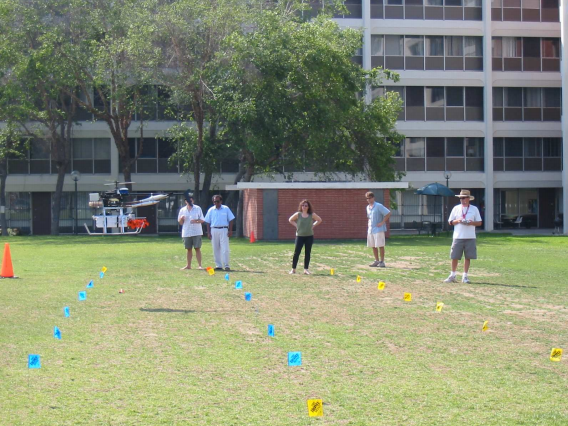
\includegraphics[width=0.3\textwidth]{figure1-1.1.png}}
%	\hspace{1cm}
%	\subfigure[]{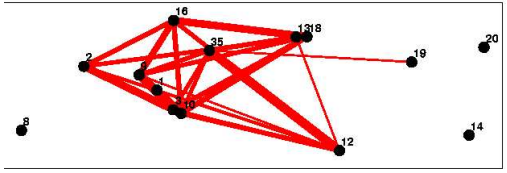
\includegraphics[width=0.3\textwidth]{figure1-1.2.png}}

%	\subfigure[]{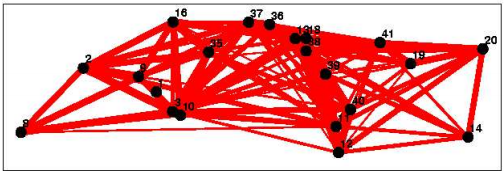
\includegraphics[width=0.3\textwidth]{figure1-1.3.png}}		
%	\bicaption[fig:SRR]{这里将出现在插图索引中}{中文题图}{Fig}{English caption}
%\end{figure*}
\begin{figure*}[!htbp]
	\begin{multicols}{2}
		
		\begin{center}
			\subfigure[直升机集中式控制拓扑网络]{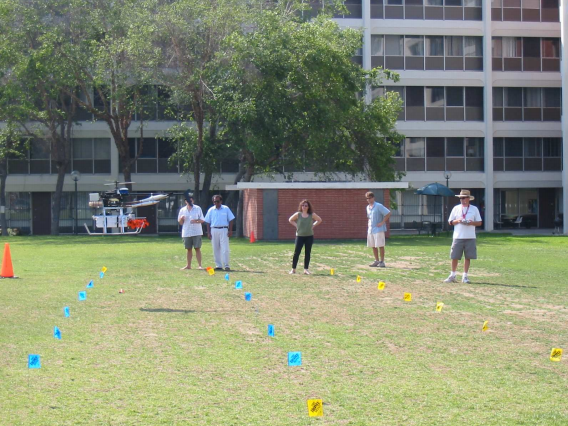
\includegraphics[width=6cm,height=4.8cm]{figure1-1.1.png}}
		\end{center}
		\begin{center}
			\subfigure[修复前的拓扑网络]{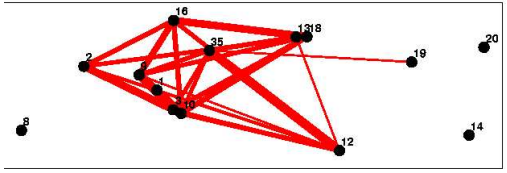
\includegraphics[width=5cm,height=1.7cm]{figure1-1.2.png}}
		\end{center}
		\begin{center}
			\subfigure[修复后的拓扑网络]{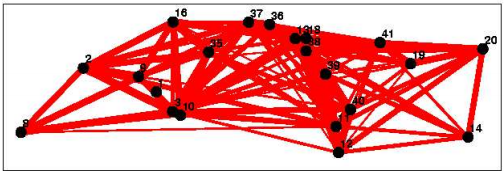
\includegraphics[width=5cm,height=1.7cm]{figure1-1.3.png}}
		\end{center}
	\end{multicols}
	\bicaption[fig:SRR]{利用无人机机进行集中式控制拓扑网络的直接自修复算法}{利用无人机机进行集中式控制拓扑网络的直接自修复算法}{Fig}{Autonomous deployment and repair of a sendor network using an unmanned aerial vehicle}
\end{figure*}

文献\parencite{Auto-holeDetection}中针对传感器网络覆盖问题进行了自修复的研究。文中主要针对网络覆盖中可能出现的空洞进行探测并修复。在算法执行过程中每个传感器节点与其他节点交换信息,多次交换信息后每个节点可以获得一个以它自身为中心的x-hop的邻居列表。即每一个节点能够获得拓扑网络中所有其他节点的信息,并计算出每个节点距离自己的跳数。如果出现空洞,则节点会根据自己的邻居列表选出一条修复路径,然后从所有的路径中选择一条效率最高的路径执行自修复。该算法需要每个节点都能够获得其他节点的信息,通信量比较大,且对每个节点的存储空间有所要求。若实现大规模节点的自修复则算法的时间和空间复杂度比较大,算法实现效率较低。

文献\parencite{Zhang2006Motion}针对多机器人编队网络的运动同步性进行自修复。当多机器人编队网络中出现机器人故障或者通信失效时,可能会影响整个网络的运动同步性。此时文中算法采用临时扩大机器人通信范围的方式,使得编队中所有机器人能够共享信息,从而直接选出合适的修复机器人进行自修复。修复过程如图1-2所示。
\begin{figure*}[!htbp]
	\begin{multicols}{2}
		\begin{center}
			\subfigure[]{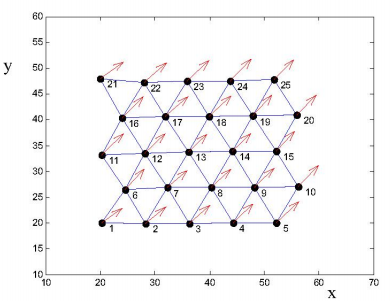
\includegraphics[width=6cm, height=4cm]{figure1-2.a.png}}
		\end{center}
		\begin{center}
			\subfigure[]{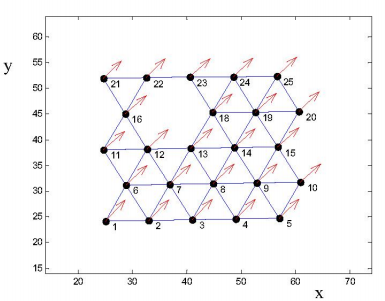
\includegraphics[width=6cm,height=4cm]{figure1-2.b.png}}
		\end{center}
		\begin{center}
			\subfigure[]{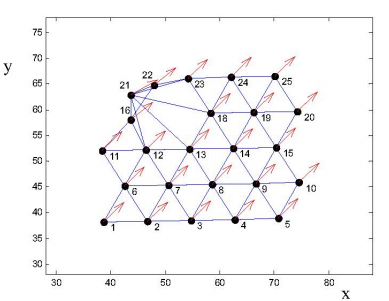
\includegraphics[width=6cm,height=4cm]{figure1-2.c.png}}
		\end{center}
		\begin{center}
			\subfigure[]{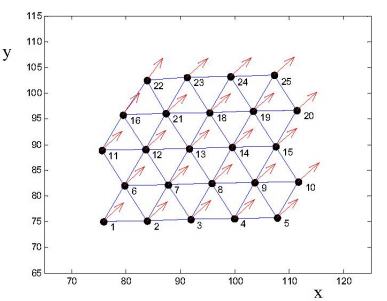
\includegraphics[width=6cm,height=4cm]{figure1-2.d.png}}
		\end{center}
	\end{multicols}
	\bicaption[fig:SRR]{多机器人编队网络运动同步性直接自修复}{多机器人编队网络运动同步性直接自修复}{Fig}{Directly self-healing for multi-robot formation motion synchronization.}	
\end{figure*}
由于出现机器人缺失后需要临时扩大机器人的通信范围,因此,算法不能算是完全分布式。并且多机器人的编队规模要收到传感器的最大通信距离的限制,不可能实现大规模机器人的编队控制,并且同样通信时间以及复杂度要随着编队规模的扩大呈指数型增长。

\subsection{密度自修复算法}
密度自修复算法主要应用在大量机器人进行自组装,形态生成或者区域覆盖等任务中。系统中的节点能够感知自身所处位置的密度,以此作为依据执行自修复算法,最终能够能够根据系统要求取得合理分布。文献\parencite{arbuckle2010self}中,作者仿照生物学纳米分子间信息交流的方式,研究了多智能体自主形态生成问题。在系统中已知一个几何形状,然后解析出几何形状的边集合,节点的有序集合。通过大量统一结构、统一编程的微小机器人执行分布式的形态生成算法可以构建出任意指定的形状。并且算法具有一定的容错机制,能够针对机器人失效,进行自修复。如图1-3所示。
\begin{figure}[!htbp]
	\centering
	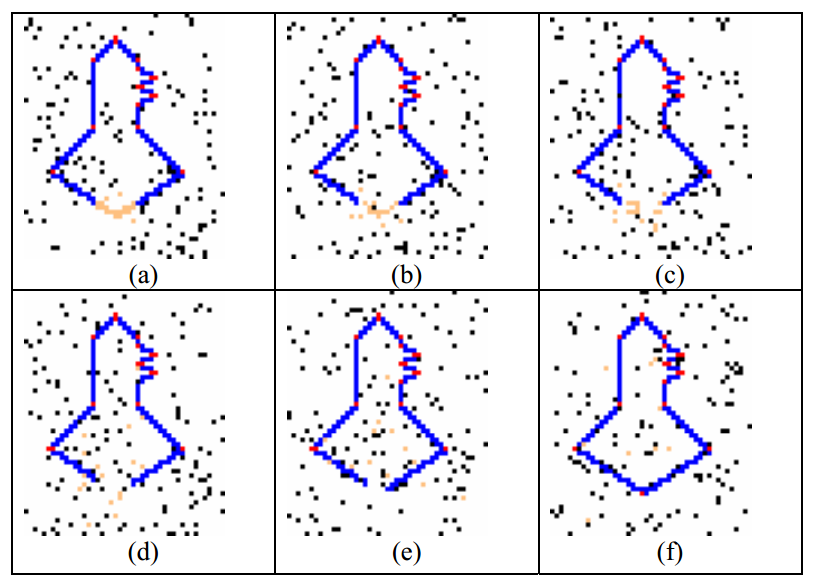
\includegraphics[width=10cm,height=6cm]{figure1-3.png}
	\bicaption[fig:SRR]{形态生成过程中机器人失效后的自修复}{形态生成过程中机器人失效后的自修复$^{[ ]}$}{Fig}{The structure recovers from the damage and self-repairs$^{[ ]}$}
\end{figure}
然而此算法的自修复过程具有一定的负面效应。即当机器人数量比较多,信息共享不完全时可能在系统中复制出两个完全一样的形状。

在文献\parencite{derbakova2011decentralized}中,作者研究了群机器人有效覆盖特定区域的算法。该算法能够实现群机器人针对某一区域的覆盖,并能对覆盖失效的情况进行自修复。系统中存在一个网关,负责所有机器人之间通信的中转。每个机器人通过与邻居通信间接与网关链接。在已知感兴趣区域的形状之后,机器人根据自身位置,结合密度信息执行分散算法,最终能够均匀覆盖该区域。并且在区域内某些机器人被移除后,系统能够自动感知缺失,并通过网关进行路径规划,调度其他机器人重新均匀覆盖此区域。如图1-4所示。
\begin{figure*}[!htbp]
	\begin{tabular}{cccc}
			\subfigure[]{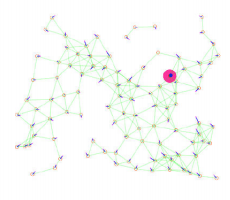
\includegraphics[width=4cm,height=5cm]{figure1-4.a.png}} &
			\subfigure[]{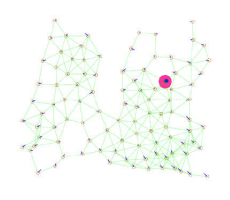
\includegraphics[width=4cm,height=5cm]{figure1-4.b.png}} &
			\subfigure[]{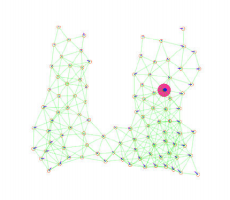
\includegraphics[width=4cm,height=5cm]{figure1-4.c.png}} &
			\subfigure[]{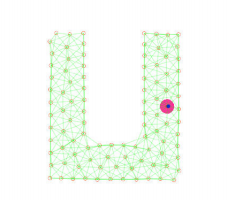
\includegraphics[width=4cm,height=5cm]{figure1-4.d.png}} \\
			\subfigure[]{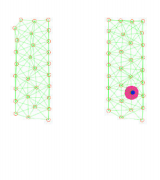
\includegraphics[width=4cm,height=5cm]{figure1-4.e.png}} &
			\subfigure[]{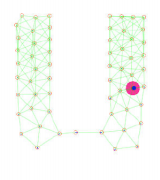
\includegraphics[width=4cm,height=5cm]{figure1-4.f.png}} & 
			\subfigure[]{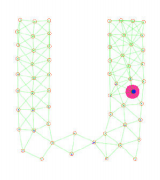
\includegraphics[width=4cm,height=5cm]{figure1-4.g.png}} &
			\subfigure[]{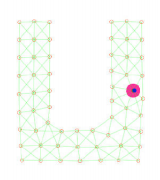
\includegraphics[width=4cm,height=5cm]{figure1-4.h.png}} \\
	\end{tabular}
	\bicaption[fig:SRR]{多移动机器人区域覆盖网络连接自修复算法}{多移动机器人区域覆盖网络连接自修复算法}{Fig}{Coverage and repair algorithm for multi-robot systems}
\end{figure*}
\subsection{递归自修复算法}
递归自修复算法利用节点或机器人之间局部交互和网络拓扑切换实现自修复。在文献\parencite{abbasi2009movement}中Abbassi等人针对无线传感器执行器网络(Wireless Sensor and Actor Networks, WSANs)中节点失效影响网络连通性的问题,提出了DARA(Distributed Actor Recovery Algorithm)算法。DARA算法针对不同的网络拓扑分为DARA-1C和DARA-2C两个版本。DARA-1C算法用于维持和修复网络的一阶连通性。算法通过心跳机制检测网络中的节点丢失。当节点出现丢失时从丢失节点的邻居中根据节点的度、离缺失节点的距离大小、自身ID号等条件选取最佳候选修复节点。网络中每个节点维持二跳邻居信息,主要针对网络中割点(cut-vertex)丢失导致网络分裂成两个或多个部分的问题进行修复。如图1-5所示。
\begin{figure*}[!htbp]
	\centering
	\begin{tabular}{ccc}
		\subfigure[]{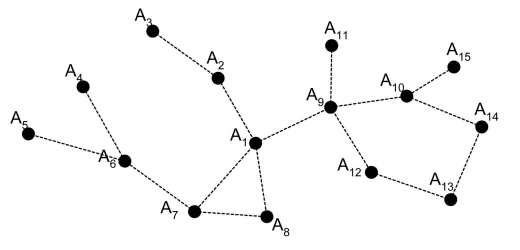
\includegraphics[width=5cm,height=3cm]{figure1-5.a.png}}
		\subfigure[]{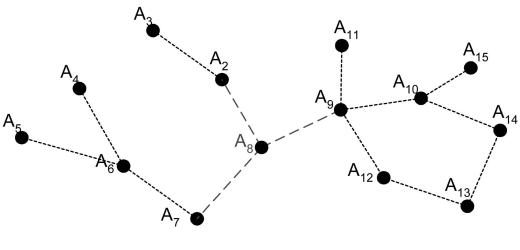
\includegraphics[width=5cm,height=3cm]{figure1-5.b.png}}
		\subfigure[]{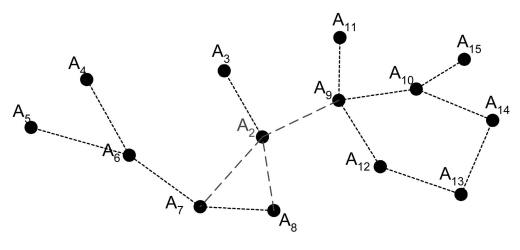
\includegraphics[width=5cm,height=3cm]{figure1-5.c.png}}
	\end{tabular}
	\bicaption[fig:SRR]{使用DARA-1C算法实现传感器网络连接自修复}{使用DARA-1C算法实现传感器网络连接自修复}{Fig}{Using DARA-1C to repair the connectivity of WSANs}
\end{figure*}

DARA-2C算法目的是维持网络的2阶连通性。可以实现网络外围节点丢失的自修复。算法的实现方式与DARA-1C类似,但主要是针对网络边缘节点进行自修复,目的是防止出现割点(cut-vertex)。修复算法只考虑是否维持2阶连通性。修复过程如图1-6所示。
\begin{figure}[!htbp]
	\centering
	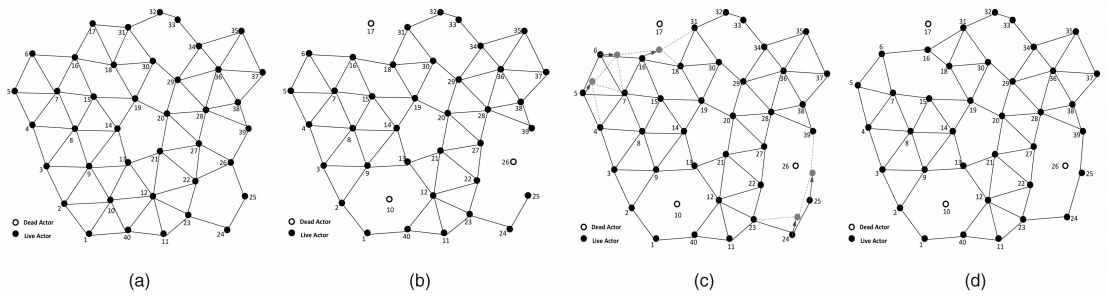
\includegraphics[width=15cm,height=4cm]{figure1-6.png}
	\bicaption[fig:SRR]{使用DARA-2C算法实现传感器网络2阶连通性自修复}{使用DARA-2C算法实现传感器网络2阶连通性自修复}{Fig}{Using DARA-2C to repair 2-connectivity of WSANs}
\end{figure}

在文献\parencite{younis2010localized}中,同样针对传感器网络连通性问题,Younis等人提出了RIM(Recovery through Inward Motion)自修复算法。该算法主要是在节点出现缺失之后,缺失节点的所有邻居节点全部向缺失节点的位置移动,直至重新建立连接。缺失节点的邻居节点移动后若如出现新的空缺则由其邻居继续执行RIM算法进行自修复,直至整个网络保持连通。如图1-7所示。该算法只考虑网络的连通性,不考虑拓扑结构的变化。
\begin{figure}
	\centering
	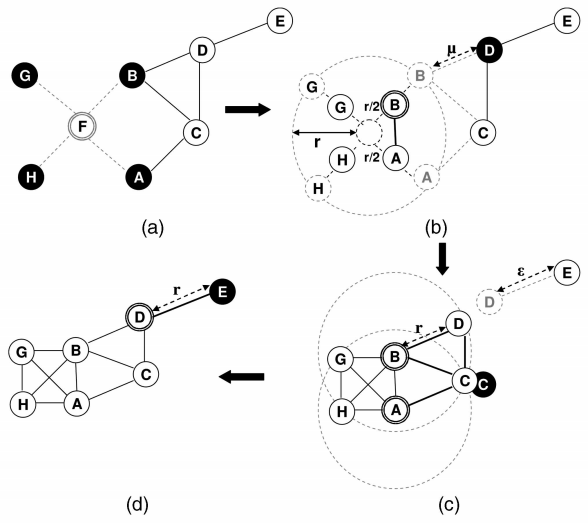
\includegraphics[width=9cm,height=8cm]{figure1-7.png}
	\bicaption[fig:SRR]{RIM算法自修复过程}{RIM算法自修复过程}{Fig}{The self-healing process of RIM algorithm}
\end{figure}

综上所述,前人关于自修复的算法几乎都是针对网络的联通性。然而类似于多机器人协同搬运这样的任务,需要多机器人能够保持特定的队形并且对编队的运动同步性要求较高。显然上述算法都无法适用于针对多机器人编队运动同步性的自修复。因此如何设计一种性能良好的针对多机器人编队网络运动同步性的自修复算法是值得思考和亟需解决的问题。

\section{本文研究内容及组织框架}
本文针对多机器人编队网络中存在机器人缺失,从而导致整个编队运动同步性下降的问题,提出了一种分布式的递归自修复算法。该算法能够实现同步性改善全局最优,通过在编队网络中构建稳定的梯度分布可以找到一条实现同步性改善全局最优的修复路径,并且该修复路径包含修复机器人个数最少,机器人运动的总距离最短。针对本文算法,不仅利用仿真验证了算法的理论可行性和有效性,而且还设计了包括多机器人空间定位系统,通信系统,运动控制系统在内的自修复实验平台。在此平台下开展了实验,验证了算法的现实可行性和可操作性。

本文主要贡献如下:\\
\indent 1) 提出了一种分布式的多机器人编队自修复算法。该算法在编队中出现机器人缺失后不仅修复了编队队形还能够实现同步性改善全局最优。\\
\indent 2) 在本文算法中引入梯度,并设计了一中新的梯度扩散与更新机制,从而实现同步性改善全局最优的同时保证修复路径最短,修复机器人个数最少。\\
\indent 3) 设计了仿真验证算法在同步性改善、修复机器人个数、修复机器人运动距离等指标的考量。\\
\indent 4) 设计了多机器人编队自修复实验平台。平台包括基于Vicon的多功能可扩展的空间定位系统、多机器人的通信系统以及机器人底层运动控制系统。

本文各章节简介如下:\\
\indent 第一章,\\
\indent 第二章,\\
\indent 第三章,\\
\indent 第四章,\\
\indent 第五章,\\




\chapter{编队网络模型和拓扑分析}
\label{chap:2}

\section{机器人编队网络模型}
在多机器人编队控制过程中,每个机器人个体都具有自主行动能力。尤其在实现分布式控制算法时,每个个体机器人需要具有独立的决策与执行能力。因此,机器人个体运动模型对编队的控制至关重要。另外在应用编队控制算法对整个编队系统进行控制从而实现特定任务时,对整体编队网络拓扑模型的掌握也是必不可少。编队网络拓扑模型是对整体编队网络拓扑分析与拓扑控制的基础\supercite{张飞2010}。

\subsection{机器人个体运动模型}
假设在$N$维空间内,机器人$i$的位置和速度分别表示为$p_i \in R^N$和$v_i \in R^N$。则机器人个体运动模型可以表示如下:\\
\begin{equation}
	\left\{
	\begin{aligned}
		\dot{p_i} & = v_i \\
		\dot{v_i} & = u_i^e + u_i^o
	\end{aligned}
	, i=1,2,\dots,n,
	\right.
\end{equation}
其中$u_i^e$表示外部对机器人的控制输入,$u_i^o$表示其他机器人对机器人$i$的影响。$u_i^e$可简单表示为:\\
\begin{equation}
	u_i^e = f(p_i,v_i), i=1,2,\dots,n
\end{equation}
若考虑障碍环境中,则$u_i^e$可表示为:\\
\begin{equation}
	u_i^e = f_a(p_i,v_i) + f_r(p_i,v_i), i=1,2,\dots,n
\end{equation}
其中,$f_a(p_i,v_i)$为目标对机器人的吸引力,$f_r(p_i,v_i)$为障碍物对机器人的排斥力。如果已知目标点的位置$T$和机器人当前位置的期望速度$v(t)$,则$f_a(p_i,v_i)$可以表示为:\\
\begin{equation}
	f_a(p_i,v_i) = a_a(T-p_i) + a_m(v(t)-v_i), i=1,2,\dots,n
\end{equation}
$a_a,a_m$分别为位置和速度的增益系数,且满足$a_a,a_m > 0$。

假设环境中存在一球形障碍物,其中心点位于$O$,半径为$r_0$,则排斥力$f_r(p_i,v_i)$可表示为:\\
\begin{equation}
	f_r(p_i,v_i) = \begin{cases}
		\frac{a_0}{{(\lvert\lvert p_i-O \rvert\rvert -r_0)}^2} \cdot \vec{r}_t, & \lvert\lvert O-p_i \rvert\rvert \leq r_0 + R_s \\
		0, &  \lvert\lvert O-p_i \rvert\rvert > r_0 + R_s
	\end{cases}
\end{equation}
其中$a_0$为排斥系数,$R_s$为人为设置的障碍物有效作用半径。$\vec{r}_t$为排斥力的方向,即$\vec{r}_t = \vec{Op_i}/\lvert\lvert\vec{Op_i}\rvert\rvert$。

\subsection{多机器人编队网络拓扑模型}
本文的拓扑结构采用基于图论的网络拓扑。假设机器人编队中有$n$个机器人,$n$个机器人组成的编队网络用$G=(V,E)$表示,其中$V$表示图中节点的集合,$E$表示节点间边的集合。每个节点$v_i\in V, i=1,2,\dots,n$表示机器人$i$, $(v_i,v_j)\in E, i,j=1,2,\dots,n$表示机器人$i,j$之间的链接。利用矩阵$A=(a_{ij}),a_{ij} \in R^{n \times n}$表示网络拓扑的耦合关系,其中\\
\begin{equation}
	a_{ij}=a_{ji} =
	\begin{cases}
		1, & (v_i,v_j) \in E \\
		0, & (v_i,v_j) \notin E
	\end{cases}
	, i,j = 1,2,\dots\dots,n, i \neq j
\end{equation}
$a_{ij} = a){ji} = 1$ 表示机器人$i,j$之间存在有效链接,否则不存在链接。耦合矩阵对角线上的元素$a_{ij} = -\sum_{i=1,i \neq j}^n a_{ij}$。规定与机器人$i$存在有效连接的机器人属于机器人$i$的邻居。则定义机器人$i$的邻居集合$N_e(i)$为:\\
\begin{equation}
	N_e(i) = \left\{ \forall j, j \neq i \wedge a_{ij}=1 \right\}
\end{equation}
机器人$i$的度为:\\
\begin{equation}
	d_i = \sum_{j \in N_e(i)} a_{ij}
\end{equation}
由此可知,耦合矩阵对角线上的元素$a_{ii} = -d_i$。

多机器人编队网络拓扑多采用$K$邻居模型\supercite{xue2004number}描述。在K邻居模型中,每个机器人的度$d_i \leq K, i=1,2, \dots ,n$。图2-1展示了几种常见的$K$邻居网络拓扑模型。

\begin{figure*}[!htbp]
	\centering
	\begin{tabular}{lr}
		\subfigure[K=3]{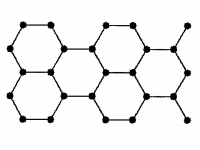
\includegraphics[width=5cm,height=4cm]{chapter2/figure2-1a.png}} &
		\subfigure[K=4]{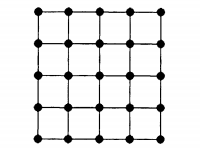
\includegraphics[width=5cm,height=4cm]{chapter2/figure2-1b.png}} \\
		\subfigure[K=6]{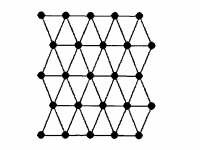
\includegraphics[width=5cm,height=4cm]{chapter2/figure2-1c.png}} &
		\subfigure[K=8]{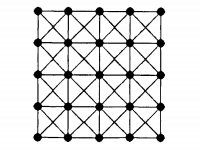
\includegraphics[width=5cm,height=4cm]{chapter2/figure2-1d.png}} \\
	\end{tabular}
\end{figure*}

\include{tex/example}
\include{tex/faq}
\include{tex/summary}

%\cite{\bibitem{\thesis.bib}}
%\bibliography{bib/thesis}

\appendix	% 使用英文字母对附录编号,重新定义附录中的公式、图图表编号样式
\renewcommand\theequation{\Alph{chapter}--\arabic{equation}}	
\renewcommand\thefigure{\Alph{chapter}--\arabic{figure}}
\renewcommand\thetable{\Alph{chapter}--\arabic{table}}
\renewcommand\thealgorithm{\Alph{chapter}--\arabic{algorithm}}

%% 附录内容,本科学位论文可以用翻译的文献替代。
\include{tex/app_setup}
\include{tex/app_eq}
\include{tex/app_cjk}
\include{tex/app_log}

\backmatter	% 文后无编号部分 

%% 参考资料
\printbibliography[heading=bibintoc]

%\bibliography{bib/thesis.bib}

%% 致谢、发表论文、申请专利、参与项目、简历
%% 用于盲审的论文需隐去致谢、发表论文、申请专利、参与的项目
\makeatletter

%%
% "研究生学位论文送盲审印刷格式的统一要求"
% http://www.gs.sjtu.edu.cn/inform/3/2015/20151120_123928_738.htm

% 盲审删去删去致谢页
\ifsjtu@review\relax\else
  %# -*- coding: utf-8-unix -*-
\begin{thanks}
时光匆匆,在交大两年半的硕士生涯转眼也接近了尾声。这是一个结束,也是一个新的开始。从此,我将离开校园,用我多年积累的学识与能力到社会上披荆斩棘。回顾这段硕士学习生涯,要感谢给予我帮助和支持的人,是你们让我一路走来无愧于自己曾经的选择,有勇气面对未来。

首先要感谢我的导师陈卫东教授,从最初入学时的稚嫩与迷茫到现在能够独立完成毕业论文,这期间的锻炼与成长离不开陈老师的悉心指导。陈老师严谨的学术态度,干练的行事风格都令我受益匪浅。另外还要感谢实验室的王贺升老师,王景川老师,卢俊国老师,他们在我的科研路上都给了极大的帮助和鼓舞。

其次要感谢刘哲师兄,一直以来对我如弟弟般关怀。无论是科研上还是生活中遇到困难,他都会给我极大的关照与帮助。还要感谢实验室的一群小伙伴,有了你们枯燥的科研生活中多了很多乐趣。是你们让我在这个庞大而陌生的城市里并不感到孤独,你们是我一生最宝贵的财富。

最后感谢父母。一直以来你们对我的关怀、理解与信任是我最坚强的后盾。同时,远在他乡没能给你们更多的陪伴,我深感愧疚!

本人能力有限,论文中诸多不足之处还请各位学者批评指正。

\end{thanks}
 	  %% 致谢
\fi

\ifsjtu@bachelor
  % 学士学位论文要求在最后有一个英文大摘要,单独编页码
  \pagestyle{biglast}
  \include{tex/end_english_abstract}
\else
  % 盲审论文中,发表学术论文及参与科研情况等仅以第几作者注明即可,不要出现作者或他人姓名
  \ifsjtu@review\relax
    \include{tex/pubreview}
    \include{tex/projectsreview}  
  \else
    %# -*- coding: utf-8-unix -*-
%%==================================================
%% pub.tex for SJTUThesis
%% Encoding: UTF-8
%%==================================================

\begin{publications}{99}
    \item\textsc{\textbf{Xiangyu Fu}, Weidong Chen, Zhe Liu, Hesheng Wang}. {A Distributed Self-healing Algorithm for Global Optimal Movement Synchronization of Multi-robot Formation Network}[C]. The 14th International Conference on Intelligent Autonomous Systems. Shanghai, China,2016.(EI)
    \item\textsc{Zhe Liu, Weidong Chen, \textbf{Xiangyu Fu}, Hesheng Wang}. {A Self-Repairing Algorithm with Optimal Repair Path for Maintaining Motion Synchronization of Mobile Robot Formation}[J]. IEEE Transactions on Control Systems Technology, Revised and Re-submitted.(SCI, Regular Paper)
    \item\textsc{Zhe Liu,Jianjun Ju, Weidong Chen, \textbf{Xiangyu Fu}, Hesheng Wang}. {A Gradient-Based Self-Healing Algorithm for Mobile Robot Formation}[C]. IEEE International Conference on Intelligent Robots and Systems. Hamburg, Germany, 2015:3395-3400.(EI)
\end{publications}
	      %% 发表论文
    %# -*- coding: utf-8-unix -*-
%%==================================================
%% projects.tex for SJTUThesis
%% Encoding: UTF-8
%%==================================================

\begin{projects}{99}
    \item 国家自然科学基金重点项目(60934006):"基于远程通信和传感器网络的多自主体协调控制"
\end{projects}
  %% 参与的项目
  \fi
\fi

% \include{tex/patents}	  %% 申请专利
% \include{tex/resume}	  %% 个人简历

\makeatother

\end{document}
